% !TeX encoding = UTF-8
% !TeX root = ../main.tex
\chapter{Implementácia grafického komponentu}

\section {Práca s Existujúcimi SVG}
Kreslenie grafických komponentov býva náročné pri zložitejších schémach. Snap.svg knižnica umožňuje načítať a používať existujúci .svg súbor.  


\section{Inkscape}

V stručnosti postup krokov na vytvorenie jednoduchého SVG súboru v Inkscape: 
\begin{enumerate}
	\item Začína sa otvorením Inkscape a vybratím File | New z menu. Vyberie sa default. 
	Na ľavej strane
\end{enumerate}

\section{Definovanie id SVG}
\section{Zoznam id SVG atributov vyuzite v priklade}





\section{Príklad vytvorenia grafického komponentu v Inkscape}

Nakreslenie jednotlivých častí komponentov prečerpávacej stanice bolo realizované pomocou ľavého bočného panela. Prečerpávacia stanica sa skladá z potrubí, indikátora úrovne hladiny vody, motora, a symbolu rotora čerpadla. Ako je možné vidieť na obrázku  \ref{picture1}.  


\begin{figure}[H]
	\begin{center}
		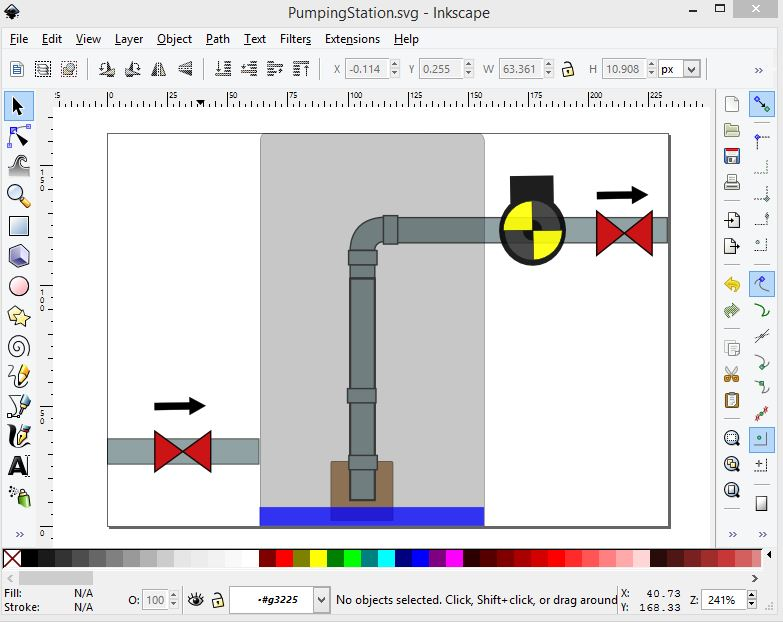
\includegraphics[width=0.7\linewidth] {obrazky/pump1.jpg}
		\caption{TODO Grafické prostredie programu Inkscape s nakreslenou prečerpávacou stanicou}
		\label{picture1}
	\end{center}
\end{figure}
=


\section{Definovanie id SVG}

Pre ovládanie JavaScriptom je nutné si pozrieť jednotlivé jedinečné identifikačné názvy. V SVG sú označované ako id. Zistenie id je pomerne jednoduché. Klikneme pravým tlačidlom na daný komponent, ktorého id chceme vedieť, a potom na Objekt Properties.

Po kliknutí sa nám zobrazí okno s názvom Object Properties. 

\begin{figure}[H]
	\begin{center}
		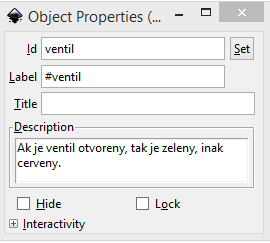
\includegraphics [width=5cm]  {obrazky/obr3.png}
		\caption{Object Properties}
		\label{picture3}
	\end{center}
\end{figure}


Z obrázka č.\ref{picture3} možno vyčítať aké je ID, predvolené sú tam napr. desc3072. Hodnoty je možné prepísať a zmeniť stlačením tlačidla Set. Pre nás je dôležitá hodnota v kolónke Label - \#ventil. 

Na ovládanie časti svg elementu cez CSS selektor je potrebné si zapamätať hodnotu Labelu.  %Spravidla hodnoty ID a Label sú rovnaké. Líšia sa iba v tom, že pri Label je pridaný znak \# pred názvom. ID je unikátny názov pre program Inkscape. 
%TODO ROZDIEL MEDZI ID A LABEL DESCRIPTION A TITTLE... TODO

Alebo ďalší spôsob zistenia id SVG časti tvarov je priamo nájsť tú hodnotu v PumpingStation.svg. Je to označené ako id="ventil".

V okne Object Properties je možné nastaviť script na animovanie. Po kliknutí na Interactivity sa zobrazia ďalšie kolónky, kde je možné zadať akciu, ktorá má nastať.  



\subsection{XML Editor}
Ďalší spôsob získania informácii o svg cez Inkscape je cez zabudovaný XML Editor.
Stlačením klávesovej skratky SHIFT + CTRL + X, alebo v hornej lište v menu vybrať ponuku Edit a na spodu je XML Editor. Následne sa zobrazí okno, ktoré je na obrázku \ref{xmlEditor}.
\begin{figure}[H]
	\begin{center}
		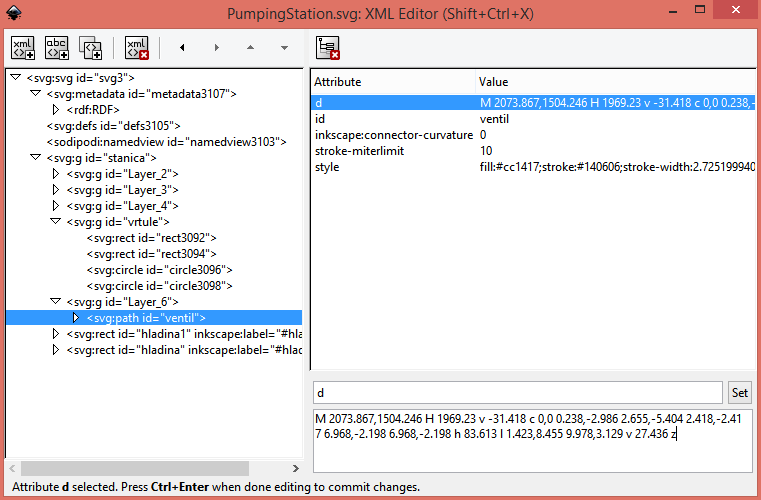
\includegraphics[width=0.7\linewidth]  {obrazky/XmlEditor2.png}
		\caption{Xml Editor v Inkscape}
		\label{xmlEditor}
	\end{center}
\end{figure}


\section{Zistenie atribútov SVG}

\subsection{Prázdna nádrž}
Prázdna nádrž je zobrazená na obrázku \ref{picture6}
Vyjadruje to, že do nádrže nevchádza tekutina. Hladina má výšku nastavenú na 9,64px. Šírka a súradnica x je rovnaká ako pri plnej nádrži. Súradnice osi y, x sú 1916,36 a 2507,84. Pri plnej nádrži sa zmení výška a os y. Pre animáciu zdvihnutia hladiny nádrže bude potrebné si zapamätať tieto súradnice. 
\begin{figure}[H]
	\begin{center}
		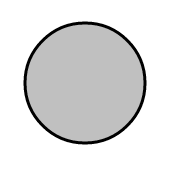
\includegraphics [height=6.5cm]  {obrazky/jednoduchyKruh.png}
		\caption{TODO Prázdna nádrž prečerpávacej stanice}
		\label{picture6}
	\end{center}
\end{figure}

\subsection{Plná nádrž}
Na obrázku č. \ref{picture5} je vykreslená plná nádrž. Hladina má súradnice x, a šírku rovnakú ako v prázdnej nádrži. Zmenila sa os y, a výška - na 1320,16 a na 605,92. 

\begin{figure}[H]
	\begin{center}
		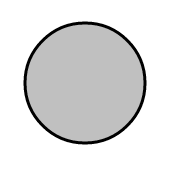
\includegraphics [height=6.5cm]  {obrazky/jednoduchyKruh.png}
		\caption{TODO Plná nádrž}
		\label{picture5}
	\end{center}
\end{figure}

V SVG súbore je to zapísané nasledovným kódom. 


\begin{lstlisting} [language=HTML]
<rect
	inkscape:label="#hladina"
	y="1320.1689"
	x="2507.8459"
	height="605.83868"
	width="797.04492"
	id="hladina"
	style=
		...
        >
</rect>

\end{lstlisting}


%%%%%%%%%%%%%%%%%%%%%%%%%%%%%%%%%%%%%%%%%%%%%%%%%%%%%%%%%%%%%%%%%%%%%%%%%%%%%%%%=
%
%Parametre ako stroke, fill, a iné sa dajú meniť prostredníctvom FUNKCIE attr v Snap API. … TODO
%%%%%%%%%%%%%%%%%%%%%%%%%%%%%%%%%%%%%%%%%%%%%%%%%%%%%%%%%%%%%%%%%%%%%%%%%%%%%%%%%=
%
%TODO POPIS SURADNICOVEHO SYSTEMU VEDIET VYSVETLIT SUVISLOST MEDZI DPI A PIX SURADNICAMI. .TODO
%
%
%TODO MIERKY OBRAZKOV ZJEDNOTIT
%TODO aj ich lokalizaciu v dokumente
%TODO









%










\section{Integrácia grafického komponentu pre dynamické ovládanie SVG objektu}

Súborová štruktúra príkladu: 
\begin{itemize}
	\item index.html 
	\item PumpingStation.js
	\item PumpingStation.svg
	\item TestPumpingStation.js
	\item exec.js 
\end{itemize}

\subsection{HTML súbor}
Do HTML súboru index.html pridáme párový tag $<$svg$>$. Na toto miesto sa neskôr vykreslí SVG načítané zo súboru cez JavaScript. Môže sa tu uviesť i celý kód SVG obrázka. V prípade, že nebude v dokumente dané kde presne sa nachádza SVG tag tak sa pridá na najbližšie voľné miesto. 
\subsection{Kód}
\begin{lstlisting}
<svg 
	id="svgStanica" 
	viewBox="0 0 750 600" 
	width="40%" 
	height="40%"> 
</svg>
\end{lstlisting}

\subsection{Vysvetlenie kódu}
\begin{itemize}
\item  \textbf{id} - jedinečný identifikátor, cez ktorý meníme vlastnosti.
\item 	\textbf{viewBox} - je virtuálne okno, ktorým sa užívateľ uvidí svg obrázok. Je atribút, ktorý povoľuje špecifikovať danú množinu grafických komponentov, aby sa zobrazili v daných súradniciach x, y a šírke, výške. Hodnoty atribútov v viewBox sú štyri čísla - min-x, min-y, width a height. 
\item 	\textbf{width} a \textbf{height} je šírka a výška. Hodnoty atribútov je možné uviesť relatívne v percentách, alebo absolútne v pixloch. 
\end{itemize}

Musíme sa uistiť, aby sa načítali všetky JavaScriptové knižnice, pred spustením funkcií. To zabezpečíme pridaním  onload do tagu $<$body$>$. 
\begin{lstlisting}
	<body onload="onPageLoad();">
\end{lstlisting}

A ešte jedna vec pri HTML súbore - TODO. 
\begin{lstlisting}[language = HTML]
  <script type="text/javascript" src="../js/snap.svg-min.js">
  </script>
  <script type="text/javascript" src="PumpingStation.js">
  </script>
\end{lstlisting}


\section{PumpingStation.js}
TODO
V súbore PumpingStation.js sú funkcie na animovanie.. TODO
\subsection{onPageLoad()}
onPageLoad() sa spustí pri načítaní tela HTML súboru index.html. Funkcia spustí funkciu PumpingStation(). Prvý parameter je udaný konkrétny svg súbor, ktorý chcem načítať. Druhý parameter je id tagu svg, ktorý je v html. TODO

\begin{lstlisting}
function onPageLoad() {
	PumpingStation("PumpingStation.svg", "#svgStanica" );
}
\end{lstlisting}

\subsection{PumpingStation(par1, par2)}

Funkcia inicializuje daný svg súbor, a vykreslí ho. 
Parametre pre PumpingStation sú názov svg súboru, a id, ktoré sa nachádza v tagu $<$svg$>$ html súbore.

\begin{lstlisting}
var PumpingStation = function(nazovFileSVG, nameHTMLidSVG) {
	paper = Snap(nameHTMLidSVG);
	Snap.load(nazovFileSVG, function (f) {
		paper.append(f);
	});
};
\end{lstlisting}

\textbf{paper} - globálna premenná. TODO REFERENCIA NA PLOCHU ... Vytvorí plochu na  kreslenie, alebo  wraps existujúci SVG element. Ako parametre môžu byť buď šírka, výška, alebo DOM element. Napríklad Snap(600, 800), alebo Snap("\#svgStanica"), resp Snap(). 

\textbf{load} - TODO funkciu z knižnice Snap. Cez ňu TODO načítam  svg súbor. Ako parametre funkcie je názov súboru svg, prípadne môže byť prázdny, ak TODO nenačítavam súbor, ale beriem ho priamo z html súboru. Druhý parameter je funkcia, v ktorej TODO volám funkciu na zobrazenie obsahu svg súboru do daného tagu svg s  id, ktorý bol daný pri funkcii paper.  Na plochu TODO ho zobrazím pomocou príkazu append. TODO

\subsection{Tank}
Zanimovanie stúpania a klesania hladiny nádrže. 
\begin{lstlisting}
var Tank = {
	idTank: "#hladina",
	tank: function(){
		return  paper.select(this.idTank);},
	animateComponentTank: function(fillPerc) {
		if (fillPerc === undefined || fillPerc < 0) {
			fillPerc = 0;
		}
		var perHeight = 600 * (fillPerc / 100);
		var perY = 1912 - perHeight;
		this.tank().animate  (	{
			height: perHeight,
			y: perY
		}, 800);
		return console.log("animacia tanku " + fillPerc);
	}
};
\end{lstlisting}
%TODO PRESTYLIZOVAT VYHODIT RODY MOJE TODO
%TODO 
Vytvorila som objekt Tank medzi jeho atribúty patria: idTank, funkcia tank, a animateComponentTank. IdTank - je stringové - je to id, ktoré som získala zo svg súboru, alebo cez Inkscape ako Label. Funkcia tank - vyberie daný objekt, ktorý chcem ovládať. Pomocou Tank.tank() môžem volať funkcie z Snap knižnice. 

Zanimovanie tanku je realizované v funkcii animateComponentTank - kde parametrom je v percentách udané o koľko sa ma zdvihnúť hladina nadrze. 
Využívam funkciu animate. Kde v prvom parametri - mením výšku a os y. Hodnotu perHeight je výška 600, ktorú vynásobím percentom o ktoré sa ma posunúť. PerY je hodnota, o ktorú sa posuniem po y-osi. Je vypočitaná ako 1912 co je y prázdnej nádrže a je od nej odpočítaná hodnota výšky. 
Ďalší parameter pri funkcii animate() je rýchlosť animácie vyjadrená v milisekundách.

\subsection{Ventil}

\begin{lstlisting}
var Valve = {
	idValve: "#ventil",
	valve: function (){ return paper.select(this.idValve);},
	colorValve: "red",
	changeIsOpen: function (isOpened) {
		isOpened = (isOpened) ? 0 : 1;
		this.colorValve = (isOpened) ?   "red" : "green";
		this.valve().attr({fill: this.colorValve});
		return;);
	}
}
\end{lstlisting}

Farba sa dá zmeniť aj príkazom 

\begin{verbatim}
Valve.valve().attr({fill: “green”});.
\end{verbatim}

Názov farby môže byť uvedený slovne, alebo ako RGB. 

Zmena farby Valve - \begin{verbatim} this.valve().attr  ({fill: this.colorValve}); \end{verbatim}


%\section{TODO TRANSFORM}
TODO TRANSFORM .. TODO